\documentclass{article}

\usepackage{amssymb,amsfonts,amsmath,amsthm}
\usepackage{mathtools}
\usepackage{bm}
\usepackage{bbold}
\usepackage{pgfplots}
\pgfplotsset{width=7cm,compat=1.8}
\usepackage[margin=60pt]{geometry}

% Codons
\newcommand{\e}{\mathrm{e}}
\begin{document}
From the difference in energy of folded and unfolded states ($\Delta G$), the probability of being folded $p(\Delta G)$ is:
\begin{equation*}
p(\Delta G) = \dfrac{1}{1 + e^{\beta \Delta G(\mathbb{S}) }}, \text{ where }
\Delta G = G_{\mathrm{F}}(\mathbb{S}) - G_{\mathrm{U}}(\mathbb{S}) \text{ and $\beta$ is the inverse temperature}.
\end{equation*}

The selection coefficient of a mutant sequence is:
\begin{equation*}
s  = \dfrac{p(\Delta G') - p(\Delta G)}{p(\Delta G)} \simeq \dfrac{ \e^{\beta \left( \Delta G - \Delta G' \right) } - 1}{ \e^{- \beta \Delta G }}.
\end{equation*}

\begin{center}
	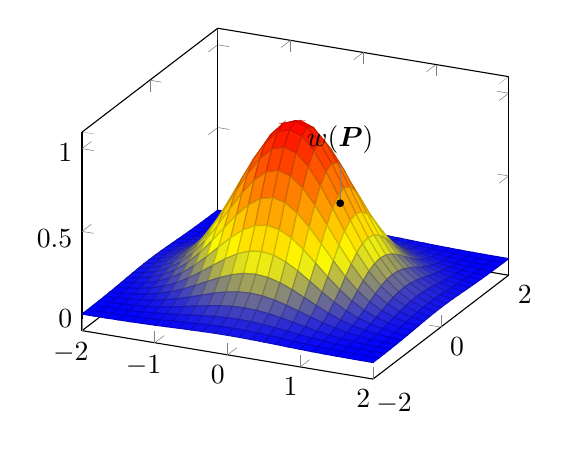
\begin{tikzpicture}
		\begin{axis}
		\addplot3[surf,domain=-2:2,domain y=-2:2] 
		{exp(-( x^2 + y^2) )};
		\node[circle,inner sep=1pt,fill=black,pin=90:$w(\bm{P})$] 
		at (axis cs:0.5,0.25,0.5) {};
		\end{axis}
	\end{tikzpicture}
\end{center}
\begin{equation*}
\bm{P}  = \sum_{1 \leq i \leq n} \bm{P_i}.
\end{equation*}
\begin{equation*}
w(\bm{P}) \propto \e^{ - \left| \bm{P} \right|^2 }
\end{equation*}
\begin{equation*}
s  = \dfrac{w(\bm{P'}) - w(\bm{P})}{w(\bm{P})}
\end{equation*}
\end{document}